\documentclass[11pt]{article}
\usepackage{csvsimple}
\usepackage{dcolumn}
\usepackage{setspace}
\usepackage{tabularx}
\usepackage[export]{adjustbox}
\usepackage{graphicx}
\usepackage{geometry}
\usepackage{subfigure}
\usepackage{lscape}
\usepackage{flafter}  % Don't place floats before their definition
\usepackage{bm}  % Define \bm{} to use bold math fonts
\usepackage{amsmath}
\usepackage{amsfonts}
\usepackage{amssymb}
\usepackage{mathtools}
\usepackage{MnSymbol}
\usepackage{url}
\usepackage{natbib}
%\usepackage{fullpage}
\bibliographystyle{cbe}
\citestyle{aa}
\usepackage{algorithm}
\usepackage[noend]{algpseudocode}
%\usepackage[vlined,algochapter,ruled]{algorithm2e}
%\usepackage[vlined,ruled]{algorithm2e}
%\SetKwComment{Comment}{$\triangleright\ $}{}

\algnewcommand\algorithmicforeach{\textbf{for each}}
\algdef{S}[FOR]{ForEach}[1]{\algorithmicforeach\ #1\ \algorithmicdo}
\algnewcommand\algorithmicswitch{\textbf{switch}}
\algnewcommand\algorithmiccase{\textbf{case}}
\algnewcommand\algorithmicdefault{\textbf{default}}
\algdef{SE}[SWITCH]{Switch}{EndSwitch}[1]{\algorithmicswitch\ #1\ \algorithmicdo}{\algorithmicend\ \algorithmicswitch}%
\algdef{SE}[CASE]{Case}{EndCase}[1]{\algorithmiccase\ #1}{\algorithmicend\ \algorithmiccase}%
\algdef{SE}[DEFAULT]{Default}{EndDefault}[1]{\algorithmicdefault\ #1}{\algorithmicend\ \algorithmicdefault}%
\algtext*{EndSwitch}%
\algtext*{EndCase}%
\algtext*{EndDefault}%
\renewcommand{\algorithmicensure}{\textbf{Result:}}

\newcommand*\NEPowerset{\mathcal{P}_{\geq 1}}
\newcommand*\gap{\textrm{(--)}}
\newcommand*\NonNegReals{\mathbb{R}_{\geq 0}}

\DeclarePairedDelimiter\setsize{\lvert}{\rvert}%

\title{ \textbf{Efficient Implied Alignment}}
\author{Alex J. Washburn and Ward C. Wheeler\\
		Division of  Invertebrate Zoology\\
		American Museum of Natural History\\
		200 Central Park West\\
		New York, NY 10024-5192\\
		USA\\
		academia@recursion.ninja\\
		wheeler@amnh.org\\
		212-769-5754}
	%\date{}
\begin{document}

\maketitle
\begin{abstract}
Given binary tree $\mathcal{T}$ of $n$ leaves, each leaf containing a string of length at most $k$, and a binary string alignment function $\otimes$, an implied alignment can be generated to describe the alignment of a dynamic homology for $\mathcal{T}$.
This is done by first decorating each node of $\mathcal{T}$ with an alignment context using $\otimes$, in a post-order traversal, then, during a subsequent pre-order traversal, inferring from those internal node decorations on which edges insertion and deletion events occurred.
Previous descriptions of the implied alignment algorithm suggest a technique of ``back-propagation'' that runs in $\mathcal{O}(k^2 * n^2)$ time.
Here we describe an implied alignment algorithm that runs in \textsc{$\mathcal{O}(k * n^2)$}.
For well-behaved data, such as molecular sequences, the runtime approaches a best case runtime of \textsc{$\Omega(k * n)$}.
This reduction in the time complexity of the procedure dramatically improves its utility in generating multiple sequence alignments and their heuristic utility.
\end{abstract}
\newpage
\tableofcontents
\newpage


%\doublespacing
\section{Introduction}
Implied Alignment (IA) was proposed by \cite{Wheeler2003} as an adjunct to Direct Optimization (DO) \citep{Wheeler1996,VaronandWheeler2012} phylogenetic tree search in order to provide verification and more rapid heuristic analysis.
IA has been a component of POY \citep{Wheeleretal2015, POY5} since its inception.
A more formal description of the algorithm was presented in \cite{Wheeleretal2006}.
Although originally designed for dynamic homology \citep{Wheeler2001} analysis, the procedure was first used as a stand-alone multiple sequence analysis (MSA) tool by \cite{WhitingAetal2006} in their analysis of skink phylogenies.
Furthermore, Whiting et al. found that IA was superior (in terms of tree optimality score) to other MSA methods in both parsimony and likelihood analyses.
This observation has been repeated multiple times (e.g. \citealp{LindgrenandDaly2007, FordandWheeler2015}; summarized in \citealp{Wheeler2012}).
The use of IA as an MSA algorithm as well as its use in the ``static approximation'' procedure described by \cite{Wheeler2003b}, benefits greatly from improvements in the time-complexity we present in this paper.

In a broader context, IA is a heuristic solution to the NP-hard Tree Alignment Problem (TAP) defined by \cite{sankoff1975}.
As such, any individual IA is not guaranteed to be either optimal or unique and there may be an exponential number of equally optimal IAs for any given binary tree.

The IA algorithm presented in this paper takes a different intellectual approach to deriving alignments than the algorithm in POY.
Previous work relied on DO to first assign median states, and then later IA consumed these median states to produce the alignment.
Here we describe IA as a way to produce the alignment first without the median states from DO, and the alignment from IA can then later be consumed to produce the median states.

The algorithm uses the repeated application of a pairwise string alignment function to perform an efficient multiple string alignment for a given binary tree describing the relationships of strings.
The more similar the strings, the better the algorithm performs.
Thus, while this algorithm has general use for performing an MSA, it is especially well-suited for the alignment of biological sequences where the strings are highly similar and a binary tree describing the strings' relationship can be provided. 
We will provide an example of the IA algorithm's performance on biological data.

\section{Definition of the heuristic function}
In order for a logically consistent alignment to be inferred, there are constraints on the heuristic alignment function used to decorate the tree prior to performing the IA algorithm.
Let $\Sigma$ be a finite alphabet of symbols such that $\setsize{\Sigma} \geq 3$.
Let $\gap \in \Sigma$ be a gap symbol which will have a special meaning in the context of an alignment.
Let $\NEPowerset (\operatorname{X})$ denote the collection of non-empty subsets of $\mathrm{X}$.
Let $\Sigma_{\Gamma}$ be the alphabet of the following symbols:

\begin{align*}
  \Sigma_{\Gamma} &      = \textbf{ALIGN}  \;\;\;\;\;\,  \NEPowerset (\Sigma) \;\; \NEPowerset (\Sigma) \;\; \NEPowerset (\Sigma)
\\                & \;\, | \;\; \textbf{DELETE} \;\;     \NEPowerset (\Sigma) \;\; \NEPowerset (\Sigma)
\\                & \;\, | \;\; \textbf{INSERT} \;\;\;\, \NEPowerset (\Sigma) \;\; \quad\quad\quad\;         \;\; \NEPowerset (\Sigma)
\end{align*}

Let $\Sigma^{*}_{\Gamma}$ be the set of all finite strings over the alphabet $\Sigma_{\Gamma}$.
Let $\otimes : \Sigma^{*}_{\Gamma} \times \Sigma^{*}_{\Gamma} \rightarrow \left(\NonNegReals,\; \Sigma^{*}_{\Gamma}\right)$ be a heuristic function that returns a non-negative alignment cost and alignment context.
It is required that $\otimes$ be commutative but need not be associative.
Both of these constraints with be discussed later.
These constraints are necessary but not sufficient for a logically consistent implied alignment to be inferred on the heuristic alignment function.

\section{Definition of an example heuristic function}
We will provide an example definition of $\otimes$ in Algorithm \ref{Alg:pairwiseAlignment} sufficient for the Implied Alignment algorithm, though there are other sufficient definitions of $\otimes$.
One candidate function fitting the description of $\otimes$ can be defined by making a slight modification to the Needleman-Wunsch \citep{Needleman1970} algorithm for pairwise string alignment.
This algorithm is very similar to DO.

First, we deterministically decide which string is assigned to the top (columns) of the alignment matrix and which string is assigned to the left side (rows).
We assign the input strings based on the data they contain.
The longer string is assigned to the columns of the alignment matrix, the shorter string to the rows.
If the strings are the same length, we take the first string under the lexical ordering of their elements and assign it to the columns and assign the second string to the rows of the alignment matrix. 
In the case that the strings are identical, the alignment is trivial.
This assignment ensures the commutativity of $\otimes$, which is necessary to enforce consistency of the IA algorithm.
Additionally, the commutivitity of $\otimes$ ensures that the IA algorithm provides the same alignment results for isomorphic tree labeling (i.e. ensures label invariance).

We now apply ``wave-front'' update procedure, which is very similar to the Needleman-Wunsch procedure to align two strings.
The subsequent ``traceback,'' however, is notably modified from the original Needleman-Wunsch procedure.
The upward, leftward, and diagonal directional arrows used to produce the alignment are additionally used to tag each element as an insertion, deletion, or alignment event, respectively. 
The pre-order traversal performed later will consumed the tagged information when merging alignment contexts.
Storing this information for each element of the pairwise alignment result allows a more efficient generation of a multiple string alignment.
This additional tagging detail is the key difference between previous alignment methods and that presented in this paper.

The example $\otimes$ presented in Algorithm \ref{Alg:pairwiseAlignment}  is of $\Theta\left( k^2 \right)$ complexity in both time and space, where $k$ is the length of the longer string.
For clarity, this example function is presented as a modification of the well understood Needleman-Wunsch algorithm, however this tagging approach can be incorporated into more sophisticated pairwise string alignment algorithms.
For instance, by using the method described by \cite{Ukkonen1985}, this algorithm's runtime could be improved to average case $\mathcal{O}\left( k * \log k \right)$ time in general, and near linear time on sequences of high similarity.
Additionally, by using the method described by \cite{Hirschberg1975}, this algorithm can be further improved to use $\mathcal{O}\left( k \right)$ space.

Note that $\sigma$ presented in throughout the pseudocode below can represent a more complex metric, such as using affine or logarithmic affine gap costs. For usage see Algorithms \ref{Alg:pairwiseAlignment},  \ref{Alg:matrixDefinition}, and \ref{Alg:matrixTraceback}.

\begin{algorithm}
  \caption{Example $\otimes$ definition}\label{Alg:pairwiseAlignment}
  \begin{algorithmic}[1]
    \Require{$lhs, \; rhs \in \Sigma_{\Gamma}^{*}$ }
    \Ensure{$\Sigma_{\Gamma}^{*}$}
    \Function{$\otimes$}{$\textit{lhs}, \textit{rhs}$}
      \newline
      \Comment{Conditionals here are required to ensure commutivity of $\otimes$.}
      \If    {$\textit{lhs} = \textit{rhs}$}
        \State \Return $\textit{lhs}$
      \ElsIf {$\textit{lhs} < \textit{rhs}$}
        \State \Return $\Call{matrixTraceback}{\sigma, \textit{lhs}, \textit{rhs}}$
      \Else
        \State \Return $\Call{matrixTraceback}{\sigma, \textit{rhs}, \textit{lhs}}$
      \EndIf
    \EndFunction
  \end{algorithmic}
\end{algorithm}

\begin{algorithm}
  \caption{Generate the alignment matrix of $\otimes$}\label{Alg:matrixDefinition}
  \begin{algorithmic}[1]
    \Require{$lesser, longer \in \Sigma_{\Gamma}^{*}$}
    \Require{$\sigma \colon \left(( \Sigma_{\Gamma}, \Sigma_{\Gamma}\right) \rightarrow \left(\NonNegReals, \Sigma_{\Gamma} \right)$}
    \Require{$i \, \in \left[-1, \; \vert \textit{lesser} \,\;\vert - 1 \right] \subset \mathbb{Z}$}
    \Require{$j    \in \left[-1, \; \vert \textit{longer} \,  \vert - 1 \right] \subset \mathbb{Z}$}
    \Ensure{($\NonNegReals$, $\mathbf{Dir}$, $\Sigma_{\Gamma}$)}
    \Function{matrixDefinition}{$\textit{lesser}, \textit{longer}, \sigma, i, j$}
      \If   {$i < 0 \lor j < 0$} \Comment{Outside of matrix is infinite cost}
        \State \Return $\left( \infty, \nwarrow, \textbf{--} \right)$
      \ElsIf{$i = 0 \land j = 0$} \Comment{Handle the origin}
        \State \Return $\left( 0, \nwarrow, \textbf{--} \right)$
      \ElsIf{$j \neq 0 \land \textit{longer}_{j-1}      = \textbf{--}$} \Comment{Preserve input gap}
        \State $\left(\textit{leftCost}, \_, \_ \right) \gets \Call{matrixDefinition}{\textit{lesser}, \textit{longer}, \sigma, i, j - 1}$
        \State \Return $\left( \textit{leftCost}, \leftarrow, \textbf{--} \right)$
      \ElsIf{$i \neq 0 \land \textit{lesser}_{i-1} \,\; = \textbf{--}$} \Comment{Preserve input gap}
        \State $\left(\textit{aboveCost}, \_, \_ \right) \gets \Call{matrixDefinition}{\textit{lesser}, \textit{longer}, \sigma, i, j - 1}$
        \State \Return $\left( \textit{aboveCost}, \uparrow, \textbf{--} \right)$
      \Else \Comment{General recursive case}
        \State $x \gets \sigma \left(           \textit{longer}_{j-1}, \textit{lesser}_{i-1} \right)$
        \State $y \gets \sigma \left(           \textit{longer}_{j-1}, \quad\quad\quad \textbf{--} \right)$
        \State $z \gets \sigma \left( \quad\quad\quad\;\, \textbf{--}, \textit{lesser}_{i-1} \right)$
        \State $\left( minCost, minDir, minElem \right) \gets \Call{getMinimal}{x, y, z}$
        \If {$\left( \textit{minDir}, \textit{minElem} \right) = \left( \nwarrow, \textbf{--} \right)$} \Comment{Aligned gap is insertion}
          \State \Return $\left( minCost, \leftarrow, \textbf{--} \right)$
        \Else
          \State \Return $\left( minCost, minDir, minElem \right)$
        \EndIf
      \EndIf
    \EndFunction
  \end{algorithmic}
\end{algorithm}

\begin{algorithm}
  \caption{Consume the alignment matrix of $\otimes$, returning the alignment and cost}\label{Alg:matrixTraceback}
  \begin{algorithmic}[1]
    \Require{$lesser,\; longer \in \Sigma_{\Gamma}^{*}$}
    \Require{$\sigma \colon \left( \Sigma_{\Gamma}, \Sigma_{\Gamma}\right) \rightarrow \left(\NonNegReals, \Sigma_{\Gamma} \right)$}
    \Ensure{($\NonNegReals$, $\Sigma_{\Gamma}^{*}$)}

    \Function{matrixTraceback}{$\textit{lesser}, \textit{longer}$}
      \State $\left( i, j \right) \gets \left( \vert \textit{lesser} \;\vert - 1,\; \vert \textit{longer} \;\vert - 1 \right)$
      \State \Return $\left( alignedCost, \_, \_ \right) \gets \Call{matrixDefinition}{\textit{lesser}, \textit{longer}, \sigma, i, j}$
      \State $alignedStr \gets \left[ \,\right]$
      \While{$\left( i, j \right) > \left( 0, 0 \right)$}
        \State $\left( \_, dirArrow, elem \right) \gets \Call{matrixDefinition}{\textit{lesser}, \textit{longer}, \sigma, i, j}$
        \Switch{$\textit{dirArrow}$}
          \Case{$\leftarrow$}
            \State $\left( i, j\right) \gets \left( i \quad\;\;, j - 1       \right)$
            \State $nextElement \gets \textbf{DELETE} \;\;   elem \;\; \textit{longer}_{j-1}$
          \EndCase
          \Case{$\uparrow$}
            \State $\left( i, j\right) \gets \left( i - 1      , j \quad\;\; \right)$
            \State $nextElement \gets \textbf{INSERT} \;\;\; elem \hspace{1.9cm} \textit{lesser}_{i-1}$
          \EndCase
          \Case{$\nwarrow$}
            \State $\left( i, j\right) \gets \left( i - 1      , j - 1       \right)$
            \State $nextElement \gets \textbf{ALIGN} \quad\; elem \;\; \textit{longer}_{j-1} \;\; \textit{lesser}_{i-1}$
          \EndCase
        \EndSwitch
        \State $alignedStr \gets nextElement + alignedStr$
      \EndWhile
      \State \Return $\left(alignedCost, alignedStr \right)$
    \EndFunction
  \end{algorithmic}
\end{algorithm}

\begin{algorithm}
  \caption{Get the minimal directional matrix context from the $3$ inputs}\label{Alg:getMinimal}
  \begin{algorithmic}[1]
    \Require{$\left(\;\;diagCost,\;\,diagElem \right) \in \left(\NonNegReals, \Sigma_{\Gamma} \right)$}
    \Require{$\left(\, rightCost,   rightElem \right) \in \left(\NonNegReals, \Sigma_{\Gamma} \right)$}
    \Require{$\left(    downCost,    downElem \right) \in \left(\NonNegReals, \Sigma_{\Gamma} \right)$}
    \Require{Total ordering over directional arrows defined as: $\nwarrow \; < \; \leftarrow \; < \; \uparrow$}
    \Ensure{$\left(\NonNegReals, \Sigma_{\Gamma} \right)$}
    \Function{getMinimal}{$ \, \left(\;\;diagCost,\;\,diagElem \right)$\newline\hspace*{3.85cm}
                          $,\, \left(\, rightCost,   rightElem \right)$\newline\hspace*{3.85cm}
                          $,\, \left(    downCost,    downElem \right)$\newline\hspace*{4cm}}
      \State \Return $minimumBy \; \left(\lambda \left(c, \_, d \right) \rightarrow \textbf{comparing}\; c \; \textbf{then} \; d\right)$\newline\hspace*{3.85cm}
      $[\, \left(\;\;diagCost, \;\,diagElem   \quad\;\;\;\;\,   ,\;      \nwarrow    \right)$\newline\hspace*{3.85cm}
      $,\, \left(\, rightCost,    rightElem \bigcup \gap, \, \leftarrow    \right)$\newline\hspace*{3.85cm}
      $,\, \left(    downCost,     downElem \bigcup \gap, \;   \uparrow \; \right)$\newline\hspace*{3.85cm}
      $]$
    \EndFunction
  \end{algorithmic}
\end{algorithm}


\section{Description of post-order traversal}
The post-order traversal (from the leaves to the root) of the binary tree $\mathcal{T}$ is a straightforward procedure.
We assign preliminary contexts and costs to each node, $n_x$, of $\mathcal{T}$.
These preliminary contexts will be consumed to assign a final string alignment in a subsequent pre-order traversal of the tree.
The post-order traversal described here is very similar to the DO post-order traversal described by \cite{Wheeler2003}, differing only in the use of $\otimes$ which captures the preliminary context of a subtree, instead of generating a preliminary median string assignment.

First, for each leaf node, $l_x$, we set $l_x.cost$ to $0$.
Additionally, if $l_x$ is of type $\Sigma^{*}$ and not of type $\Sigma^{*}_{\Gamma}$ --- i.e. if it has been decorated with a finite string of symbols from the alphabet $\Sigma$, and not it is not decorated with a finite string of preliminary contexts over the alphabet $\Sigma_{\Gamma}$ --- then we call $\Call{initializeString}{l_x.prelimString}$ to apply the transformation $\Sigma^{*} \rightarrow \Sigma^{*}_{\Gamma}$.

On each internal node, $i_x$ with children $c_l$ and $c_r$, of $\mathcal{T}$, we call $c_l$ $\otimes$ $c_r$.
The resultant \textit{prelimString} is assigned to $i_x.prelimString$, and the sum of the $c_l.cost$ and $c_r.cost$ is assigned to $i_x.cost$.
By performing this operation in a post-order traversal over $\mathcal{T}$, we propagate the preliminary contexts and costs returned from the calls to $\otimes$ up the tree from the leaves to the root.

After performing the post-order traversal, each internal node contains the preliminary context information and the cost for the entire subtree.
Consequently, when the post-order traversal is complete, the root node contains the preliminary context information of the full leaf set of strings.
In the pre-order traversal, we will consume this preliminary context to perform an (efficient) alignment on the strings.

Because the post-order traversal can be performed using any valid  $\otimes$ definition, the complexity of the post-order traversal is dependent on the complexity of the heuristic alignment function used.
Let the complexity of $\otimes$ be defined as $H(k)$, where $k$ is the maximum string length of the leaf labels of the tree $\mathcal{T}$.
Then post-order traversal runs in $\mathcal{O}(H(k) * n)$ time and space, where $n$ is the number of leaves in the binary tree $\mathcal{T}$.
If we were to use Ukkonnen's method with the $\otimes$ described in Algorithm \ref{Alg:pairwiseAlignment}, the post-order traversal would run in $\mathcal{O}(k * \log  k * n)$ average case time and space.

\section{Pseudocode of post-order traversal}

\begin{algorithm}
  \caption{Post-order Traversal}\label{post-order}
  \begin{algorithmic}[1]
    \Require{$inputString \in \Sigma^{*}$ }
    \Ensure{$\Sigma_{\Gamma}^{*}$ }
    \Function{initializeString}{$\textit{inputString}$}
      \State $i \gets \vert\textit{inputString} \;\vert - 1,$
      \While{$i \geq 0$}
        \State $\textit{inputString}_i \gets \textbf{ALIGN} \; \left\{ \textit{inputString}_i\right\} \left\{ \textit{inputString}_i \right\} \left\{ \textit{inputString}_i \right\}$
      \EndWhile
      \Return $\textit{inputString}$
    \EndFunction

    \Require{A binary tree decorated with leaf labels $inputString \in \Sigma_{\Gamma}^{*}$ }
    \Ensure{A binary tree decorated with internal labels $prelimString \in \Sigma_{\Gamma}^{*}$ }
    %    \Procedure{post-order(n)}{}
    \Function{post-order}{$\textit{node}$}
      \If   {isLeaf ( $\textit{node}$ )}
        \State $\textit{node.cost} \gets 0$
%        \If {isOfType ($\Sigma^{*}$, $\textit{node.prelimString}$ )}
%          \State $\textit{node.prelimString} \gets \Call{initializeString}{node.prelimString}$
%sy        \EndIf
      \Else
        \State $\textit{lhs}  \gets \Call{post-order}{\textit{node.children.first}}$
        \State $\textit{rhs}  \gets \Call{post-order}{\textit{node.children.second}}$
        \State $\left(\textit{alignCost}, \textit{alignContext}\right) \gets \textit{lhs.prelimString} \otimes \textit{rhs.prelimString}$
        \State $\textit{node.cost} \gets \textit{alignCost} + \textit{lhs.cost} + \textit{rhs.cost}$
        \State $\textit{node.prelimString} \gets \textit{alignContext}$
      \EndIf
    \EndFunction
  \end{algorithmic}
\end{algorithm}


\section{Description of pre-order traversal for final alignments}
The pre-order traversal (from the root to the leaves) of the binary tree $\mathcal{T}$ consumes the preliminary context decorations created in the post-order traversal in order to assign final alignment decorations to each node.
First, the root node must be initialized for the pre-order traversal by assigning the final alignment as the preliminary context, replacing all deletion events in the preliminary context with insertion events.
This is required because, at the root node, deletion events originate from alignments of the left subtree and insertion events originate from alignments of the right subtree, however the origin of these events are indistinguishable at the root node.
By initializing the root node in this manner, we treat the root node consistently with the treatment of any other parent node when deriving the internal node alignments in Algorithm \ref{deriveAlignment}.

For each non-root node $n_x$, we first determine whether the current node is the left or right child of its parent.
If it is the left child, then each deletion event of the parent node's final alignment is changed to an insertion event and each insertion event is changed to a deletion event.
This is required because (as with the root node) deletion events originate from alignments of the left subtree and insertion events originate from alignments of the right subtree. 
However, we must consider the converse when referencing the parent's final alignment with a node which is the left child of it's parent for the resulting alignment to be consistent.

Once the final alignment of the parent has been correctly initialized, we proceed to assign the final alignment of the current node.
The parent's final alignment will necessarily be of greater than or equal length to the parent's preliminary context and the parent's preliminary context is also greater than or equal to than the current node's preliminary context, due to the addition of alignment gaps $\gap$ on the post-order traversal.
The resulting value assigned to the current node's final alignment will have the same length as the parental final alignment.
Since this invariant is maintained from the root node to the leaf node's final alignment assignments, all alignments will have the same length.
This constitutes a simple inductive proof that the final alignment assignment of each node will be of equal length and constitute a genuine string alignment.

The final alignment for the current node is derived by performing a ``sliding zip'' over the parent's final alignment, the parent's preliminary context, and the current node's preliminary context.
The parent's final alignment is used as the basis of the zip, .
At each step of the ``sliding zip,'' one element of the parent's final alignment will be consumed and one element of the current node's final alignment will be defined.
Additionally, at each step of the zip, one element of either the parent's preliminary context, the current node's preliminary context, or both elements will also be consumed.
The process is called a ``sliding zip'' because the elements of the parent's and current node's preliminary contexts do not have a fixed index to which they correspond to the parent's final alignment being used as the basis of the zip.
Rather, the elements of the parent's and current node's preliminary contexts ``slide'' through the zipping process, and their corresponding index with the basis is deduced dynamically.
An example alignment of this ``sliding zip'' process for two internal  nodes is shown in Figure \ref{Fig:Examplepre-order}.
Deletion events in the parental final alignment are propagated to the current node's final alignment without consuming elements of the parental or current node's preliminary contexts.
For each non-deletion element in the parental final alignment, one element from either the parent's preliminary context or the current node's preliminary context, or both elements are consumed to determine which element is added to the current node's final alignment depending on the deletion, insertion, or alignment event of the next parental preliminary context element.
However, the final alignment assignments for internal nodes and leaf nodes are defined slightly differently within the ``sliding zip.''
There are ten special cases describing how to derive each index current node's final alignment. The special cases are described in the pseudocode in Algorithm \ref{Alg:pre-order} and Figure \ref{Fig:Examplepre-order}.

%\begin{itemize}
%
%\item If the next element of the parental final alignment is a deletion event, consume the parental final alignment element and add a deletion event to the current node's final alignment.
%
%\item If the next element of the parental final alignment is an insertion or alignment event and the next element of the parental preliminary context is a deletion event, then we consume both elements and add a deletion event to the current node's final alignment.
%
%\item If the next element of the parental final alignment is an insertion event and the next element of the parental preliminary context is an alignment event, then we consume both elements along with the next element of the current node's preliminary context and add the consumed element of the current node's preliminary context to the current node's final alignment.
%
%\item If the next element of the parental final alignment is an insertion event and the next element of the parental preliminary context is an insertion event and we are deriving the alignment of a leaf node, then we must inspect the median value of the next element of the current node's preliminary context.
%If the median value is \textit{not} the same as the inserted value from the parental preliminary context, then we consume both the parental final alignment and the parental preliminary context elements and add a deletion event to the current node's final alignment. 
%If the median value is the same as the inserted value from the parental preliminary context or we are not deriving the alignment of a aligning a leaf node, then we consume all three elements along and add the consumed element of the current node's preliminary context to the current node's final alignment, converting a deletion event to an insertion event if the consumed element of the current node's preliminary alignment was a deletion event.
%
%\item If the next element of the parental final alignment is an alignment event and the next element of the parental preliminary context is an insertion event, then we consume both elements along with the next element of the current node's preliminary context and add the consumed element of the current node's preliminary context to the current node's final alignment.
%
%\item If the next element of the parental final alignment is an alignment event and the next element of the parental preliminary context is an alignment event, we must check if we are deriving the alignment for a leaf node.
%If we are deriving the alignment for a leaf node, then we consume both elements along with the next element of the current node's preliminary context and add the consumed element of the current node's preliminary context to the current node's final alignment.
%If we are \textit{not} deriving the alignment for a leaf node, then we consume both elements along with the next element of the current node's preliminary context and add the consumed element of the parental preliminary context to the current node's final alignment.
%
%\end{itemize}

The improvement of the implied alignment algorithm presented here compared to the original algorithm is that the additional stored information allows us to determine the final assignments in $\Theta(k * m * n)$ instead of $\mathcal{O}(k^2 * n^2)$ time. 
The aforementioned $n^2$ component occurred in previous implementations due to the use of a ``back-propagation'' technique, which required that, at each pre-order step, each new gap found in the alignment was retroactively applied to every alignment derived in a previous pre-order step.
Additionally, the $k^2$ component in the previous implementation was due to using a Needleman-Wunsch string alignment between the current node and its parent node at each pre-order step.
By saving the requisite information on the nodes during the post-order traversal, then consuming this information with the ``sliding-zip'' technique, we replace these computationally expensive operations with a much more efficient algorithm.

Let $m = \frac{a}{k}$, where $k$ is the length of the longest input string, and $a$ is the length of the root node's preliminary string decoration.
In the best case that a ``perfect alignment'' is derived, that is, that each element of all the input strings can be aligned with one of the elements of the longest input string, then $m = 1$.
In the worst case that a ``degenerate alignment'' is derived, that is, that no element of any of the input strings can be aligned with any of the elements of the longest input string, and all input strings are of equal length, then $m = n$.

In the pre-order traversal algorithm presented above, we generate an implied alignment in $\Theta(k * m * n)$ time.
We must preform a ``sliding-zip'' operation on each node in the binary tree $\mathcal{T}$, hence the factor of $n$.
The ``sliding zip'' accounts for the $k * m$ factor.

The best case runtime occurs when the length of the derived alignment is the length of the longest input string, an alignment with the minimal number of elements.
In this case, $m = 1$ and the ``sliding zip'' performed on each node performs work equal to the length of the longest input string $k$.
Hence, the best case runtime of the implied alignment algorithm is $\Omega(n*k)$ when the input strings are highly correlated and $m = 1$.

The worst case runtime occurs when the length of the derived alignment is equal to the sum of the lengths of the input strings, an alignment with the maximum number of elements.
In the worst case, $m \gg 1$, and the ``sliding zip'' performed on each node performs work equal to the length of the longest input string, $k$, times the number of input strings, $n$.
Hence, the worst case runtime of the implied alignment algorithm is $\mathcal{O}(k * n^2)$ when the input strings are independent of each other.

%I will note the similarity and difference to implied alignment derivation mentioned by Ward's previous works.


\section{Pseudocode of pre-order traversal}

\begin{algorithm}
  \caption{Pre-order Traversal}\label{pre-order}
  \begin{algorithmic}[1]
    \Require{      A binary tree decorated with leaf     labels $inputString   \in \Sigma_{\Gamma}^{*}$}
    \Require{      A binary tree decorated with internal labels $prelimString  \in \Sigma_{\Gamma}^{*}$}
    \Ensure {$\;\;$A binary tree decorated with leaf     labels $alignedString \in \Sigma_{\Gamma}^{*}$}
    \Ensure {$\;\;$A binary tree decorated with internal labels $finalString   \in \Sigma_{\Gamma}^{*}$}
    \Function{pre-order}{$\textit{node}$}
      \If    {isRoot ( $\textit{node}$ )} \Comment{Initialize the root node}
        \State $\textit{node.finalString} \gets \Call{initializeRootString}{\textit{node.prelimString}}$
      \Else
        \State $\textit{parentFinal} \;\;\; \gets \textit{node.parent.finalString}$
        \State $\textit{parentPrelim}    \, \gets \textit{node.parent.prelimString}$
        \State $\textit{childPrelim} \;\;\;\, \gets \textit{node.prelimString}$
        \If {isLeftChildOfParent($\textit{node}$)}
          \ForEach {$\textit{context} \in \textit{parentPrelim}$}
            \State \Call{reverseContext}{$\textit{context}$}
          \EndFor
        \EndIf
        \State $\textit{v} \gets$ \Call{deriveAlignment}{$isLeaf ( \textit{node} ), \textit{parentFinal}, \textit{parentPrelim}, \textit{childPrelim}$}
        \State $\textit{node.finalString} \gets \textit{v}$
      \EndIf
    \EndFunction

    \Function{initializeRootString}{$\textit{rootString}$}
      \ForEach {$\textit{context} \in \textit{rootString}$}
        \Call{deletionToInsertion}{$\textit{context}$}
      \EndFor
    \EndFunction

    \Function{deletionToInsertion}{$\textit{context}$}
      \Switch{$\textit{context}$}
        \Case{$\textbf{DELETE} \;\; \textit{m} \;\; \textit{x} \;\;$}
          \Return $\textbf{INSERT} \;\; \textit{m} \;\; \textit{x} \;\;$
        \EndCase
        \Case{$\textit{v} \;\;$}
          \Return $\textit{v}$
        \EndCase
      \EndSwitch
    \EndFunction

    \Function{reverseContext}{$\textit{context}$}
      \Switch{$\textit{context}$}
        \Case{    $\textbf{ALIGN} \quad\; \textit{m} \;\;      \textit{x} \;\; \textit{y} \;\;$}
          \Return $\textbf{ALIGN} \quad\; \textit{m} \;\;      \textit{y} \;\; \textit{x} \;\;$
        \EndCase
        \Case{    $\textbf{DELETE} \;\;   \textit{m} \;\;      \textit{x} \;\;\quad$}
          \Return $\textbf{INSERT} \;\;\; \textit{m} \;\;\quad \textit{x} \;\;$
        \EndCase
        \Case{    $\textbf{INSERT} \;\;\; \textit{m} \;\;\quad \textit{y} \;\;$}
          \Return $\textbf{DELETE} \;\;   \textit{m} \;\;      \textit{y} \;\;$
        \EndCase
      \EndSwitch
    \EndFunction
  \end{algorithmic}
\end{algorithm}


\newgeometry{top=1mm, bottom=1mm}

\begin{algorithm}
  \label{Alg:pre-order}
  \caption{Internal Node Alignment}\label{deriveAlignment}
  \begin{algorithmic}[1]
    \Function{deriveAlignment}{$\textit{isLeaf}, \textit{pAlignment}, \textit{pContext}, \textit{cContext}$}
      \State $\textit{del}   \;\;\quad \gets \textbf{DELETE}$ -- --
      \State $\textit{len}   \;\;\quad \gets$ \Call{length}{$\textit{pAlignment}$}
      \State $\textit{pcLen} \;        \gets$ \Call{length}{$\textit{pContext}$}
      \State $\textit{ccLen} \;        \gets$ \Call{length}{$\textit{cContext}$}
      \State $\left( \textit{i}, \textit{j}, \textit{k} \right) \gets \left( 0, 0, 0 \right)$
      \For{$\textit{i} < \textit{len}$}
        \If    {$\textit{j} \geq \textit{pcLen} \land \textit{k} \geq \textit{ccLen}$}
          \State $\textit{result}_i \gets \textit{del}$ \Comment{Case 0}
        \ElsIf {$\textit{k} \geq \textit{ccLen}$}
          \Switch{$\textit{pAlignment}_i$}
            \Case{$\textbf{DELETE} \;\;   \textit{m} \;\;      \textit{x} \;\;\quad$} \Comment{Case 1}
              \State $\textit{result}_i \gets \textit{del}$
            \EndCase
            \Default{} \Comment{Case 2}
              \State $\textit{result}_i \gets \textit{del}$
              \State $\textit{j} \gets \textit{j} + 1$
            \EndDefault
          \EndSwitch
        \Else
          \Switch{$\textit{pAlignment}_i$}
            \Case{$\textbf{DELETE} \;\;   \textit{m} \;\;      \textit{x} \;\;\quad$} \Comment{Case 3}
              \State $\textit{result}_i \gets \textit{del}$
            \EndCase
            \Case{$\textbf{INSERT} \;\;\; \textit{m} \;\;\quad \textit{y} \;\;$} 
              \Switch{$\textit{pContext}_j$}
                \Case{$\textbf{DELETE} \;\;   \textit{m} \;\;      \textit{x} \;\;\quad$} \Comment{Case 4}
                  \State $\textit{result}_i \gets \textit{del}$
                \EndCase
                \Case{$\textbf{INSERT} \;\;\; \textit{m} \;\;\quad \textit{y} \;\;$} \Comment{Case 5}
                  \If {$\textit{isLeaf} \land y \neq \;$\Call{getMedian}{$\textit{cContext}_k$}}
                    \State $\textit{result}_i \gets \textit{del}$
                  \Else
                    \State $\textit{result}_i \gets$ \Call{deletionToInsertion}{$\textit{cContext}_k$}
                    \State $\textit{k} \gets \textit{k} + 1$
                  \EndIf
                \EndCase
                \Case{$\textbf{ALIGN} \quad\; \textit{m} \;\;      \textit{x} \;\; \textit{y} \;\;$} \Comment{Case 6}
                  \State $\textit{result}_i \gets \textit{cContext}_k$
                  \State $\textit{k} \gets \textit{k} + 1$
                \EndCase
              \EndSwitch
              \State $\textit{j} \gets \textit{j} + 1$
            \EndCase
            \Case{$\textbf{ALIGN} \quad\; \textit{m} \;\;      \textit{x} \;\; \textit{y} \;\;$} 
              \Switch{$\textit{pContext}_j$}
                \Case{$\textbf{DELETE} \;\;   \textit{m} \;\;      \textit{x} \;\;\quad$} \Comment{Case 7}
                  \State $\textit{result}_i \gets \textit{del}$
                \EndCase
                \Case{$\textbf{INSERT} \;\;\; \textit{m} \;\;\quad \textit{y} \;\;$} \Comment{Case 8}
                  \State $\textit{result}_i \gets \textit{cContext}_k$
                  \State $\textit{k} \gets \textit{k} + 1$
                \EndCase
                \Case{$\textbf{ALIGN} \quad\; \textit{m} \;\;      \textit{x} \;\; \textit{y} \;\;$} \Comment{Case 9}
                  \If {$\textit{isLeaf}$}
                    \State $\textit{result}_i \gets \textit{cContext}_k$
                  \Else
                    \State $\textit{result}_i \gets \textit{pContext}_j$
                  \EndIf
                    \State $\textit{k} \gets \textit{k} + 1$
                \EndCase
              \EndSwitch
              \State $\textit{j} \gets \textit{j} + 1$
            \EndCase
          \EndSwitch
        \EndIf
        \State $\textit{i} \gets \textit{i} + 1$
      \EndFor
      \Return $\textit{result}$
    \EndFunction
  \end{algorithmic}
\end{algorithm}

\begin{figure}[h]
	\caption{Example pre-order alignment for two internal nodes}
	\label{Fig:Examplepre-order}
	\vspace{2ex}
	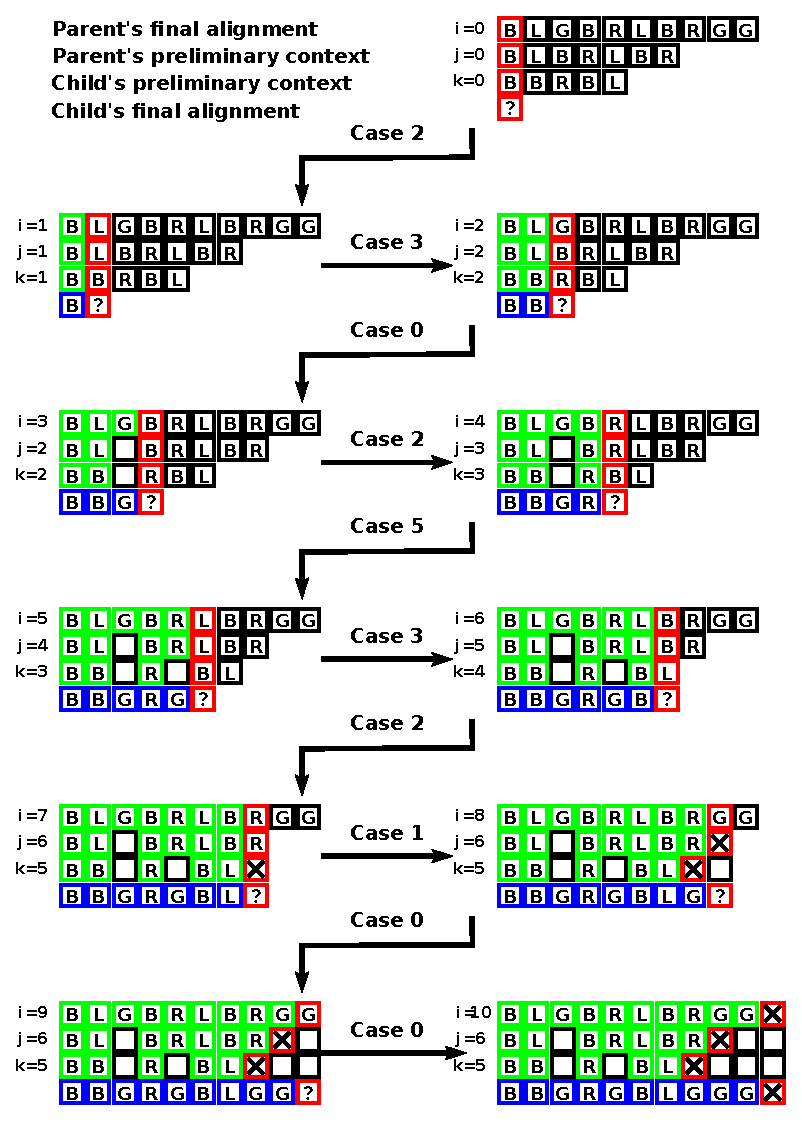
\includegraphics{example-preorder.eps}
\end{figure}

\restoregeometry

\section{Conclusion and Empirical Examples}

An example Haskell implementation of the implied alignment algorithm described above, along with a script to replicate the results discussed below can both be found here: 

\centerline{\url{https://github.com/recursion-ninja/efficient-implied-alignment}}

To explore the runtime performance of the pre-order traversal, we ran the implied alignment algorithm described in this paper on fungal and metazoan biological data sets described by \cite{GiribetandWheeler1999} and \cite{GiribetandWheeler2001} respectively.
Both full data sets consisted of a preselected tree and predetermined string alignment (i.e. including gaps).
The full leaf set of the tree was repeatedly pruned in half to produce a data set of doubling leaf set sizes.
The string alignment was repeatedly truncated, dropping the beginning and end of the alignment, taking the central slice of the correct length from each string, and then removing all the gaps from the alignment slice.
The pruned trees and truncated strings were used as progressively doubling inputs, to measure runtime scaling in terms of both leaf set size and string length.
Both biological data sets used the discrete metric $\sigma_0$ and the alphabet $\Sigma = \{\mathrm{A, C, G, T, --} \}$.

Additionally, a pathological data set was constructed to illustrate the best and worst case performance of the implied alignment algorithm.
The pathological data set consisted of balanced binary trees which repeatedly doubled in size.
The strings of the pathological data set consisted of a single symbol repeated some specified number of times.
The lengths of the strings containing many copies of a single character were repeatedly doubled in size.
The data set also used the alphabet $\Sigma = \{\mathrm {A, C, G, T, --} \}$.

The runtime scaling of this pathological data set was examined under two different metrics $\sigma_1$ and $\sigma_2$.
The former metric preferentially selects substitution events over insertion or deletion events and hence produces the ``perfect alignment.''
Conversely, the latter selects for insertion or deletion over substitution thus producing the ``degenerate alignment.''


After running each data set, we constructed an Ordinary Least Square (OLS) model with the output runtime in milliseconds as a function of dimensions $k$ and $n$.
We took the binary logarithm, $\log_{2}$, of both input dimensions as well as the output.
From there, we calculated the coefficients of each input in this equation: $\log_2(runtime) = \beta_0 + \beta_1 \log_2(n) + \beta_2 \log_2(k) + \epsilon$, where $\epsilon$ represents the estimation error.
Note that because the logarithm of the inputs was taken, we would expect $\beta_1$ to be close to $1$ for linear performance with respect to that input variable and close to $2$ for quadratic performance.
See Table \ref{Tab:Regression}.

The pathological data sets shows the stark runtime difference between the best case $\Omega(n * k)$ and worst case $\mathcal{O}(k * n^2)$ runtimes.
The OLS model empirically supports the theoretical best and worst case runtimes demonstrated by the two runs of the pathological data set as shown in Figures \ref{Fig:Best} and \ref{Fig:Worst}. % and  Tables \ref{Tab:Best} \& \ref{Tab:Worst}

The OLS model also showed that the runtime scales well for the biological data sets.
The fungal and metazoan sequence data sets demonstrate a near-linear and quasi-linear runtime with respect to the number of input strings and linear runtime with respect to string length.
The fungal data sets shows that some of the ``real world'' use cases can perform close to the theoretical best case runtime (see Figures \ref{Fig:Fungi} and \ref{Fig:Metazoa}). % and Tables \ref{Tab:Fungi} \& \ref{Tab:Metazoa}.


\begin{table}[!hbt]
\caption{Metric costs of $\sigma_0$, $\sigma_1$, and $\sigma_2$}
\label{Tab:Metrics}
\begin{minipage}{0.3\textwidth}
	\centering
	\begin{tabular}{c|ccccc}
		$\sigma_0$ & A & C & G & T & -- \\ \hline
		A  & 0 & 1 & 1 & 1 & 1  \\
		C  & 1 & 0 & 1 & 1 & 1  \\
		G  & 1 & 1 & 0 & 1 & 1  \\
		T  & 1 & 1 & 1 & 0 & 1  \\
		-- & 1 & 1 & 1 & 1 & 0
	\end{tabular}
%	\caption{Discrete}
\end{minipage}
\hfill
\begin{minipage}{0.33\textwidth}
\centering
\begin{tabular}{c|ccccc}
$\sigma_1$ & A & C & G & T & -- \\ \hline
        A  & 0 & 1 & 1 & 1 & 2  \\
        C  & 1 & 0 & 1 & 1 & 2  \\
        G  & 1 & 1 & 0 & 1 & 2  \\
        T  & 1 & 1 & 1 & 0 & 2  \\
        -- & 2 & 2 & 2 & 2 & 0
\end{tabular}
%\caption{Prefer Align}
\end{minipage}
\hfill
\begin{minipage}{0.3\textwidth}
\centering
%\begin{table}[!hbt]
%\begin{center}
\begin{tabular}{c|ccccc}
$\sigma_2$ & A & C & G & T & -- \\ \hline
        A  & 0 & 3 & 3 & 3 & 1  \\
        C  & 3 & 0 & 3 & 3 & 1  \\
        G  & 3 & 3 & 0 & 3 & 1  \\
        T  & 3 & 3 & 3 & 0 & 1  \\
        -- & 1 & 1 & 1 & 1 & 0
\end{tabular}
%\caption{Prefer InDel}
\end{minipage}
\end{table}

%\begin{table}
%\scriptsize
%\begin{minipage}{0.5\textwidth}
%\centering
%\caption{Fungi pre-order results}
%\begin{tabular}{l|l|l}%
%    \bfseries $n$ & \bfseries $k$ & \bfseries Runtime (ms)% specify table head
%    \csvreader[head to column names]{fungi-11.pre-order.csv}{}% use head of csv as column names
%    {\\\hline\csvcoliii&\csvcoliv&\csvcolv}% specify your coloumns here
%\end{tabular}
%\end{minipage}
%\hfill
%\begin{minipage}{0.5\textwidth}
%\centering
%\caption{Metazoa pre-order results}
%\begin{tabular}{l|l|l}%
%    \bfseries $n$ & \bfseries $k$ & \bfseries Runtime (ms)% specify table head
%    \csvreader[head to column names]{metazoa-11.pre-order.csv}{}% use head of csv as column names
%    {\\\hline\csvcoliii&\csvcoliv&\csvcolv}% specify your coloumns here
%\end{tabular}
%\end{minipage}
%\end{table}

%\begin{table}
%\scriptsize
%\begin{minipage}{0.5\textwidth}
%\centering
%\caption{Best case pre-order results}
%\begin{tabular}{l|l|l}%
%    \bfseries $n$ & \bfseries $k$ & \bfseries Runtime (ms)% specify table head
%    \csvreader[head to column names]{pathological-12.pre-order.csv}{}% use head of csv as column names
%    {\\\hline\csvcoliii&\csvcoliv&\csvcolv}% specify your coloumns here
%\end{tabular}
%\end{minipage}
%\hfill
%\begin{minipage}{0.5\textwidth}
%\centering
%\caption{Worst case pre-order results}
%\begin{tabular}{l|l|l}%
%    \bfseries $n$ & \bfseries $k$ & \bfseries Runtime (ms)% specify table head
%    \csvreader[head to column names]{pathological-31.pre-order.csv}{}% use head of csv as column names
%    {\\\hline\csvcoliii&\csvcoliv&\csvcolv}% specify your coloumns here
%\end{tabular}
%\end{minipage}
%\end{table}


% Table created by stargazer v.5.2.2 by Marek Hlavac, Harvard University. E-mail: hlavac at fas.harvard.edu
% Date and time: Fri, Oct 11, 2019 - 11:29:04 AM
% Requires LaTeX packages: dcolumn 
\begin{table}[!htbp] \centering 
	\caption{Regression coefficients of string count and string length on runtime} 
	\label{Tab:Regression} 
	\begin{tabular}{@{\extracolsep{5pt}}lD{.}{.}{-3} D{.}{.}{-3} D{.}{.}{-3} D{.}{.}{-3} } 
		\\[-1.8ex]\hline 
		\hline \\[-1.8ex]
		& \multicolumn{4}{c}{\textit{Dependent variable:}} \\ 
		\cline{2-5} 
		\\[-1.8ex] & \multicolumn{4}{c}{$\log_2$(Runtime)} \\ 
		& \multicolumn{1}{c}{Best} & \multicolumn{1}{c}{Worst} & \multicolumn{1}{c}{Fungi} & \multicolumn{1}{c}{Metazoa} \\ 
		\\[-1.8ex] & \multicolumn{1}{c}{(1)} & \multicolumn{1}{c}{(2)} & \multicolumn{1}{c}{(3)} & \multicolumn{1}{c}{(4)}\\ 
		\hline \\[-1.8ex] 
		$\log_2$(String count $\;n$) & 1.000 & 1.854 & 1.193 & 1.499 \\ 
		& & & & \\ 
		$\log_2$(String length $k$) & 0.920 & 0.888 & 0.753 & 1.067 \\ 
		& & & & \\ 
		\hline \\[-1.8ex]
		Observations & \multicolumn{1}{c}{25} & \multicolumn{1}{c}{25} & \multicolumn{1}{c}{42} & \multicolumn{1}{c}{42} \\ 
		Adjusted R$^{2}$ & \multicolumn{1}{c}{0.943} & \multicolumn{1}{c}{0.971} & \multicolumn{1}{c}{0.984} & \multicolumn{1}{c}{0.991} \\ 
		\hline 
		\hline \\[-1.8ex] 
	\end{tabular}
\end{table}

\newcolumntype{R}[1]{>{\raggedleft\arraybackslash}p{#1}}

\begin{figure}[h]
\centering
\begin{minipage}{0.49\textwidth}
\centering
\caption{Fungi pre-order runtime}
\label{Fig:Fungi}
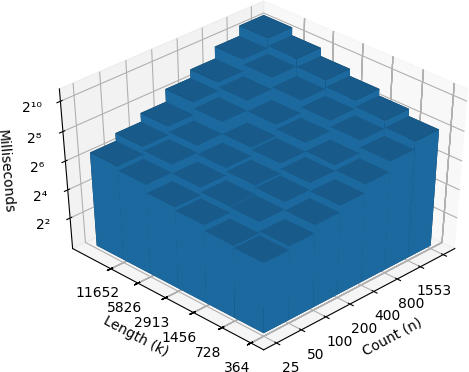
\includegraphics[width=1.05\textwidth]{fungi-preorder.png}
\end{minipage}
\hfill
\begin{minipage}{0.49\textwidth}
\centering
\caption{Metazoa pre-order runtime}
\label{Fig:Metazoa}
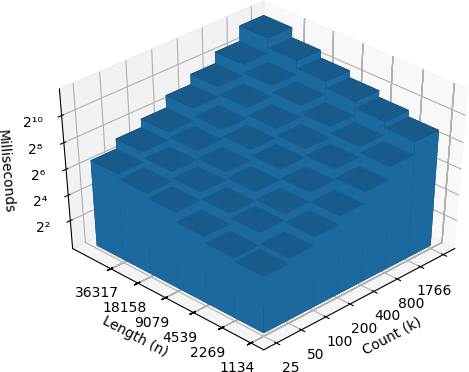
\includegraphics[width=1.05\textwidth]{metazoa-preorder.png}
\end{minipage}

\begin{minipage}{0.49\textwidth}
\centering
\caption{Best case pre-order runtime}
\label{Fig:Best}
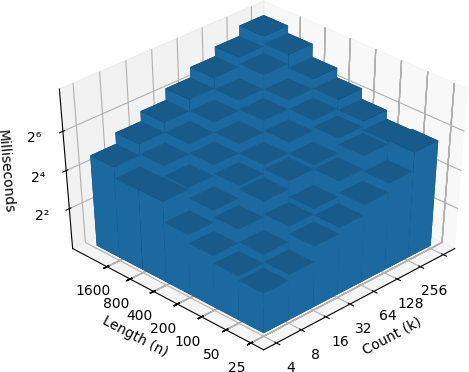
\includegraphics[width=1.05\textwidth]{pathological-12-preorder.png}
\end{minipage}
\hfill
\begin{minipage}{0.49\textwidth}
\centering
\caption{Worst case pre-order runtime}
\label{Fig:Worst}
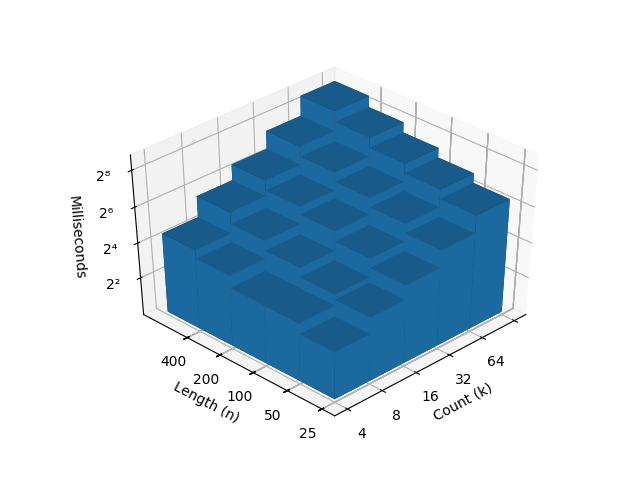
\includegraphics[width=1.05\textwidth]{pathological-31-preorder.png}
\end{minipage}
\end{figure}


\section{Why `Implied' Alignment}

The algorithm originally described by \cite{Wheeler2003} was given the name implied alignment to differentiate it from other methods (e.g. sum-of-pairs alignment) unconnected to the vertex string assignments `implied' by the binary tree on a given leaf-set. 
However, it is worth articulating exactly how the alignment we derive is \emph{implied} by the tree.
In short, it is the lack of associativity.

For the purposes of this analysis we will ignore the cost returned from the $\otimes$ and consider only the resulting alignment context.
Therefore let $\oplus : \Sigma^{*}_{\Gamma} \times \Sigma^{*}_{\Gamma} \rightarrow \Sigma^{*}_{\Gamma}$ be defined as $\otimes$ but ignoring the alignment cost of the result. If we are given a rooted binary tree $\mathcal{T} = ((A,B),(C,D))$ with leaves $A, B, C, D \in \Sigma^{*}$ then the ancestral state of the root node defined by the heuristic function $\oplus$ would be $((A \oplus B) \oplus (C \oplus D))$. 
In fact, the ancestral state of any internal node defined by $\oplus$ can be calculated by applying $\oplus$ recursively to the subtree of the internal node.
The binary structure of the tree directly implies the precedence of each application of $\oplus$ in the final result.
Since $\oplus$ need not be associative, the tree $((A,(B,C)),D)$ evaluated as $((A \oplus (B \oplus C)) \oplus D)$, is likely to yield different results.
However, since $\oplus$ is commutative, transposing any child nodes between the left and right positions of their parent will result in a tree that yields the same internal values. 
For example consider a transposed tree $\mathcal{T'}$:

\begin{align*}
  eval(\mathcal{T'}) &= eval((D,C),(B,A))
\\  &= ((D \oplus C) \oplus (B \oplus A))
\\  &= ((C \oplus D) \oplus (B \oplus A))
\\  &= ((C \oplus D) \oplus (A \oplus B))
\\  &= ((A \oplus B) \oplus (C \oplus D))
\\  &= eval((A,B),(C,D))
\\  &= eval(\mathcal{T})
\end{align*}

This commutative property and lack of an associative property is why the alignment is implied by the tree on the leaf-set under $\oplus$ and not the unique alignment on all trees for the leaf-set under $\oplus$.
Clearly, a $\oplus$ that is both commutative \emph{and} associative using the algorithm described in this paper would yield the same alignment on all trees for a given leaf-set.

String alignment is of paramount importance in phylogenetic search, though when the string alignment occurs can be a matter of contention.
Traditionally all input sequence strings are aligned first, and that alignment is held constant as a phylogenetic tree is searched for on this alignment.
A more modern method of dynamic homology has been described by \citep{Wheeler1996}, in which strings are not pre-aligned, but rather the strings are compared vertex by vertex on the current tree under consideration in the phylogentic search.
Although implied alignments are not required to identify phylogenetic trees that are heuristically `best,' they can be used in enhanced tree search heuristics during a dynamic homology search (as in POY \citealp{POY5, Wheeleretal2015}) or as the basis of a search itself as with more traditional approaches.

How a string alignment is used in a phylogenetic search leads to an important distinction in interpreting the meaning of the resulting string alignment.
When performing the traditional methodology of aligning strings then searching on the static alignment, the resulting topology of the phylogenetic search is implied by the initial alignment.
When using implied alignment to search on a dynamic homology, the alignments depend on the topology.

%See figure from this other paper Ward will note, as a good example of how Implied Alignment differs from a traditional multiple sequence alignment algorithm.

\section{Future work}
If a heuristic function $\otimes$ that was both commutative and associative and with sufficiently low error could be defined, then the iterative approximation \citep{Wheeler2003a} could be dramatically improved upon. 
Even an incredibly expensive, poly-time $\otimes$ definition would have its cost amortized over the tree-space search because the heuristic would only need to be applied once to a dynamic homology and then an implied alignment generated, which would be the same for all trees in the tree space. 
The iterative approximation would cease needing to be iterative and rather be an \emph{invariant} approximation.

\section{Acknowledgements}
We would like to thank Eric Ford, Callan McGill, Katherine St. John, and Erilia Wu for insightful discussions. This work was supported by DARPA SIMPLEX (``Integrating Linguistic, Ethnographic, and Genetic Information of Human Populations: Databases and Tools,'' DARPA-BAA-14-59 SIMPLEX TA-2, 2015-2018)
 and Robert J. Kleberg Jr. and Helen C. Kleberg foundation grant ``Mechanistic Analyses of Pancreatic Cancer Evolution''.

\newpage
\bibliography{big-refs-3}
\newpage

%\section{Appendix}
%
%\begin{table}
%	\scriptsize
%	\caption{Fungi pre-order results (milliseconds)}
%	\begin{tabular}{R{0.6cm}|R{1cm}R{1cm}R{1cm}R{1cm}R{1cm}R{1.1cm}}%
%		\bfseries $n\backslash k$ &   364 &    728 &   1456 &   2913 &    5826 &   11652 \\\hline     
%		25  &   730 &   1399 &   2072 &   2664 &    5691 &    7683 \\
%		50  &  1385 &   2214 &   3497 &   5696 &   23837 &   16300 \\
%		100  &  4133 &   5301 &   9498 &  14467 &   24514 &   34216 \\
%		200  &  7238 &  11577 &  18303 &  23809 &   57262 &   78167 \\
%		400  & 12092 &  24190 &  35627 &  66681 &  140659 &  214599 \\
%		800  & 36959 &  52147 & 101514 & 217350 &  333379 &  709528 \\
%		1553  & 86631 & 137355 & 310405 & 487501 & 1462000 & 1743000
%		\label{Tab:Fungi}
%	\end{tabular}
%	
%	%\end{table}
%	%\begin{table}
%	\scriptsize
%	\caption{Metazoa pre-order results (milliseconds)}
%	\begin{tabular}{R{0.6cm}|R{1cm}R{1cm}R{1cm}R{1cm}R{1cm}R{1.1cm}}%
%		\bfseries $n\backslash k$ &   1134 &   2269 &   4539 &    9079 &   18158 &   36317 \\\hline     
%		25  &    420 &    612 &   1068 &    3401 &    5902 &    9787 \\
%		50  &    979 &   1543 &   3074 &    8333 &   15272 &   27715 \\
%		100  &   1824 &   3668 &   7526 &   17478 &   33379 &   64810 \\
%		200  &   3874 &  12721 &  29071 &   56608 &   97899 &  187654 \\
%		400  &  14621 &  29731 &  63591 &  162526 &  347680 &  501298 \\
%		800  &  49024 &  88415 & 225158 &  503264 &  787639 & 1670000 \\
%		1766  & 194138 & 365731 & 726205 & 1533000 & 2889000 & 6925000
%		\label{Tab:Metazoa}
%	\end{tabular}
%	%\end{table}
%	%\begin{table}
%	\scriptsize
%	\caption{Best case pre-order results (milliseconds)}
%	\begin{tabular}{R{0.6cm}|R{1cm}R{1cm}R{1cm}R{1cm}R{1cm}}%
%		\bfseries $n\backslash k$ &     25 &     50 &    100 &     200 &     400 \\\hline     
%		4  &     21 &    118 &     46 &     118 &     270 \\
%		8  &     50 &     49 &    103 &     207 &     382 \\
%		16  &     54 &    130 &    203 &     400 &     887 \\
%		32  &    138 &    233 &    446 &     925 &    1786 \\
%		64  &    249 &    466 &    881 &    1769 &    3584
%		\label{Tab:Best}
%	\end{tabular}
%	%\end{table}
%	%\begin{table}
%	\scriptsize
%	\caption{Worst case pre-order results (milliseconds)}
%	\begin{tabular}{R{0.6cm}|R{1cm}R{1cm}R{1cm}R{1cm}R{1cm}}%
%		\bfseries $n\backslash k$ &     25 &     50 &    100 &     200 &     400 \\\hline     
%		4  &    127 &     60 &    165 &     244 &     604 \\
%		8  &    336 &    240 &   1223 &    1002 &    2167 \\
%		16  &    994 &    997 &   1937 &    3896 &    8369 \\
%		32  &   1726 &   3938 &   7070 &   15197 &   33148 \\
%		64  &   6743 &  13620 &  28416 &   63780 &  145712
%		\label{Tab:Worst}
%	\end{tabular}
%\end{table}

\end{document}
